\subsection{Technical Indicators}
\label{sec:TechnicalIndicators}

% Introduction
As James Chen of Investopedia puts it: ["Technical indicators are heuristic or pattern-based signals produced by the price, volume, and/or open interest of a security or contract used by traders who follow technical analysis"] \citep{Chen_2021}. These indicators are essential tools for traders and analysts to make informed decisions.
\newline
\newline
% The price chart
All technical indicators are applied to a price chart, which provides traders and investors a visual representation of historical price movements in financial markets. Price charts as illustrated in figure \ref{fig:bitcoin_price_chart}, offer insights into market trends, patterns and potential future price directions, enabling investors to make informed trading decisions. Common types of price charts include line charts, bar charts and candlestick charts, each offering a unique perspective on market dynamics. By incorporating technical indicators such as \gls{ma}, \gls{bb} and stochastic oscillators, traders can further analyse price chart patterns to identify potential entry and exit points, as well as gauge market momentum and volatility.

\begin{figure}[ht]
    \centering
    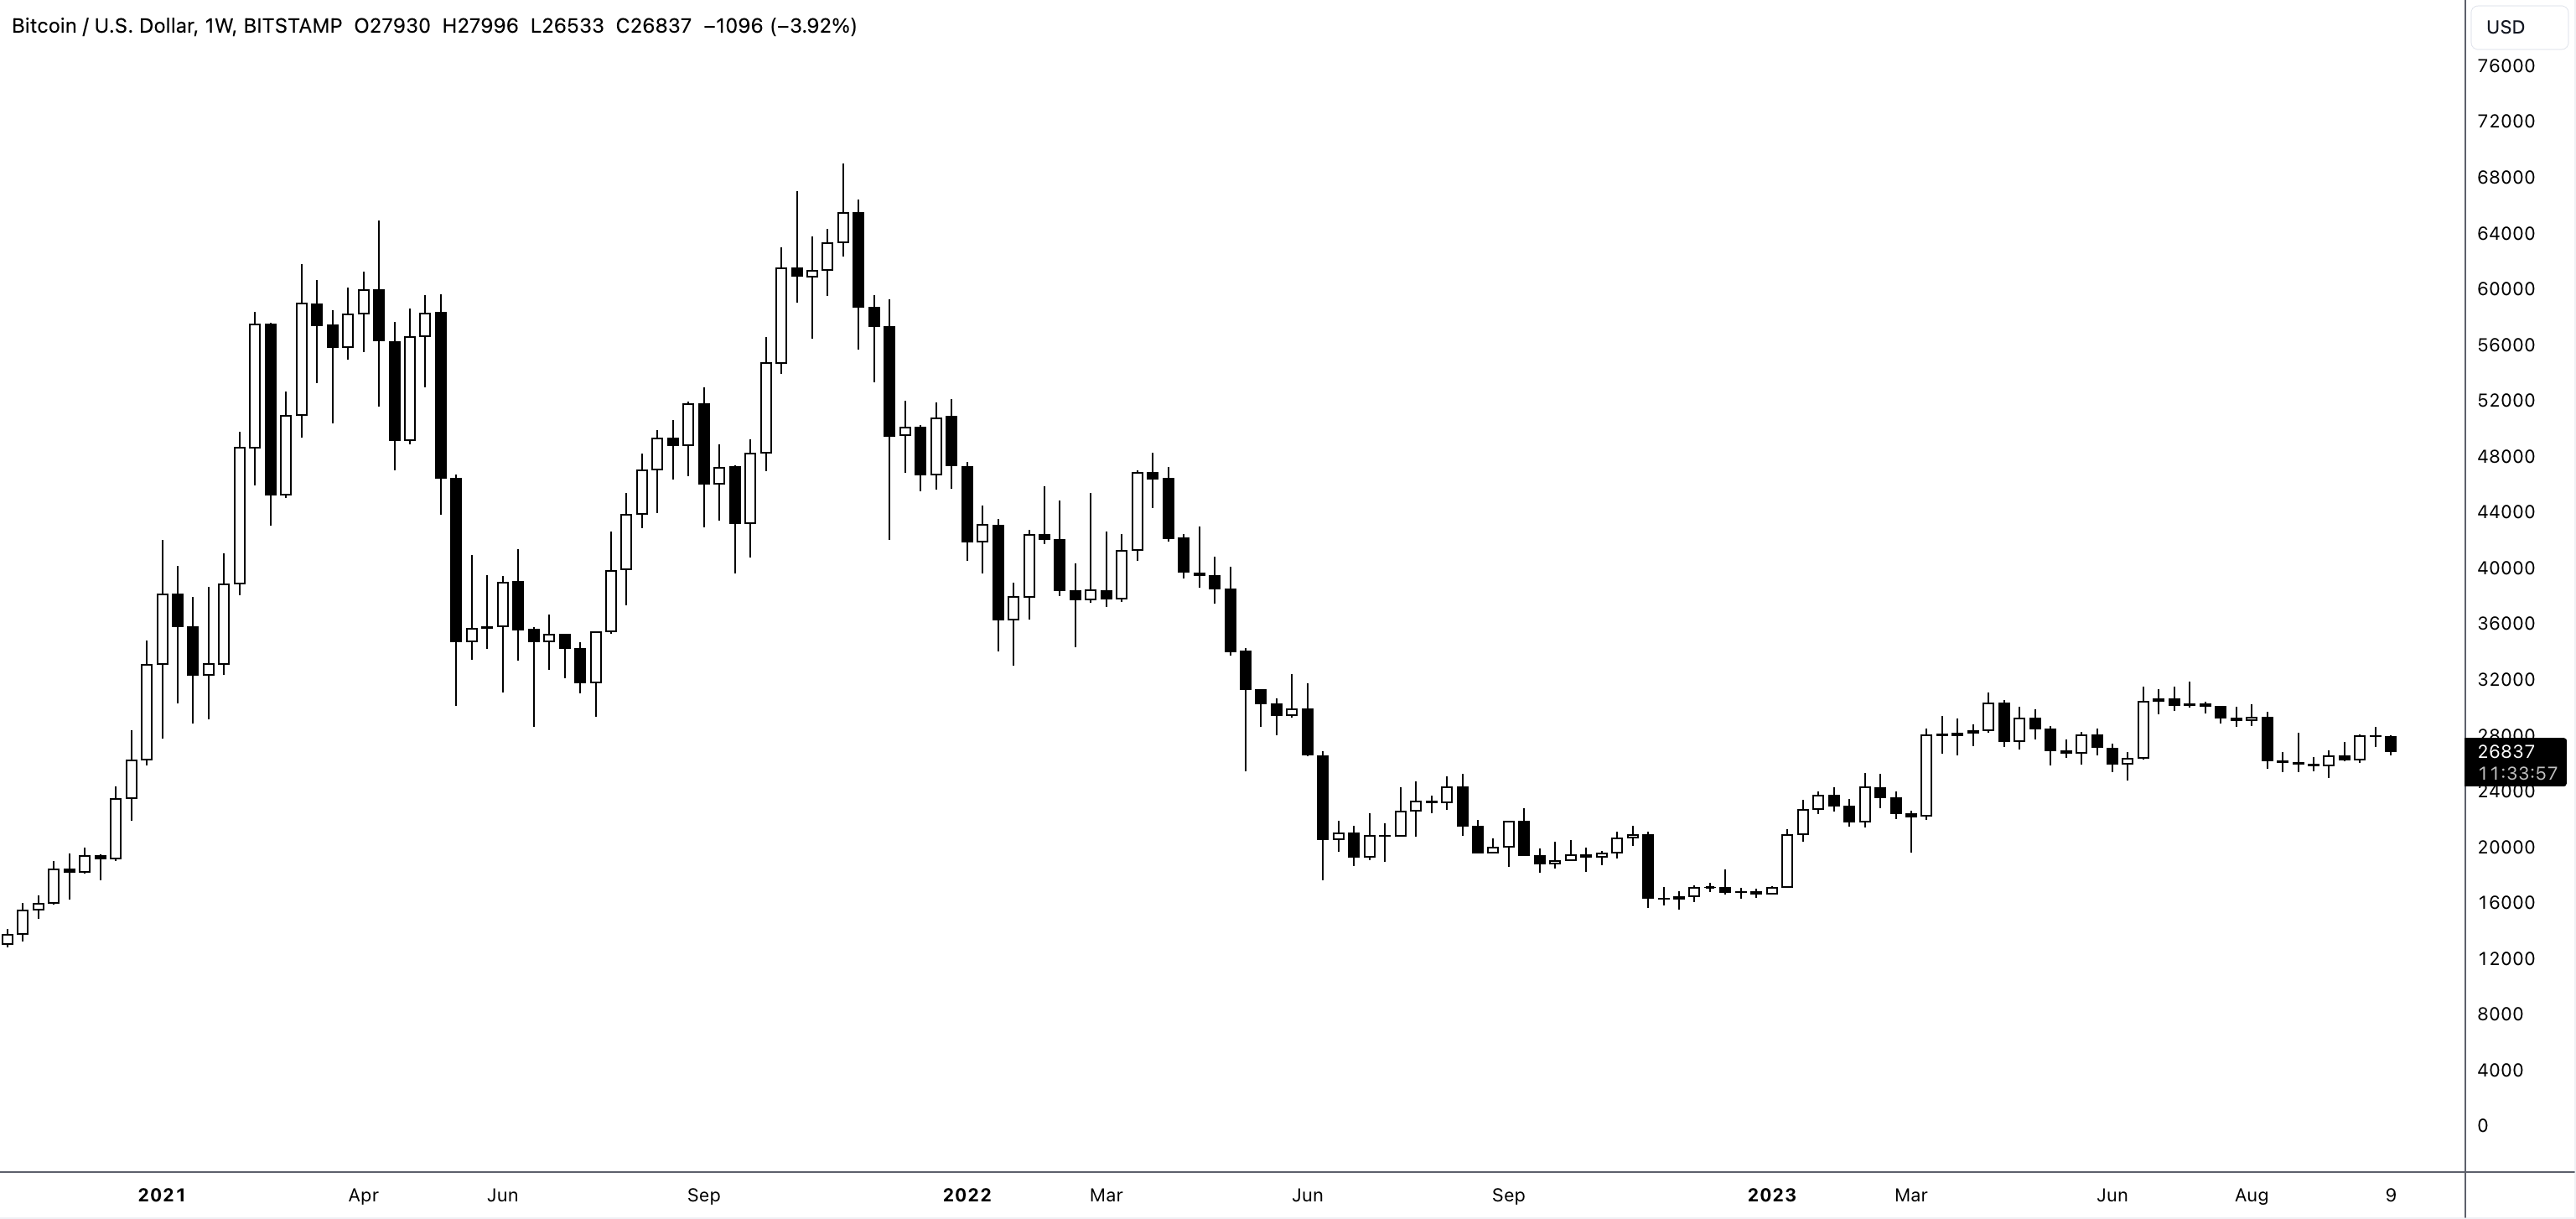
\includegraphics[width=\textwidth]{./assets/img/bitcoin_price_chart.png}
    \caption{Figure shows weekly price movements of \gls{btc} in USD as a candlestick chart from October 2020 to October 2023.}
    \label{fig:bitcoin_price_chart}
\end{figure}

\noindent
% Types of Technical Indicators
Technical indicators can be divided into two main types: momentum and lagging indicators. Momentum indicators measure the rise or fall of asset prices, helping to assess their current strength. On the other hand, lagging indicators signal market changes after they have already occurred, thus confirming the long-term trend.
\newline
\newline
Furthermore, both momentum and lagging can be further categorized into overlays and oscillators. Overlays are plottet on the price chart itself and have the same scale as the price. Examples of overlays are \gls{ma} and \gls{bb}. Oscillators, on the other hand, are indicators that osciallate between local minima and maxima and are typically plotted below the price chart. Well-known oscillators include the \gls{rsi} and the \gls{macd} \citep{Chen_2021}.

% Moving Average
\subsection{Moving Average}
\label{sub:MA}
The \gls{ma} is a technique for smoothing data points that has been used for decades, long before a general term came into use. In 1909, G. U. Yule \citep{yule1909applications} described the ["instantaneous averages"] of R. H. Hooker \citep{hooker1901correlation} as ["moving averages"]. But Yule did not adopt the term in his textbook. It came into circulation through W. I. King's book \textit{Elements of Statistical Method} in 1912 \citep{king1912elements}.
\newline
\newline
The \gls{ma} is a fundamental indicator used in technical analysis to smooth price data, reduce noise and highlight trends. Traders and investors commonly use the 50-day and 200-day \gls{ma} as important \glspl{tf} for analysis. The 50-day \gls{ma} looks at the past 50 trading days, while the 200-day \gls{ma} looks at the past 200 days. Because the \gls{ma} is based on historical price data, it is generally considered to be a lagging indicator.
\newline
\newline
There are two main types of \gls{ma}: the \gls{sma} and the \gls{ema}. The \gls{sma} calculates the arithmetic mean $\frac{1}{d}$ of the price $v_t$ over a specified time period from $t = 1, 2, \dots, d$, represented as $\text{SMA} = \frac{1}{d} \sum_{t=1}^d v_t$. On the other hand, the \gls{ema} integrates a smoothing factor $k$ to give greater weight to recent prices within the time period $d$. The calculation of the \gls{ema} can be expressed as in the equation \ref{eq:exp_moving_average}, where $k$ is denoted as $\frac{2}{d + 1}$.

\myequations{Computing the exponential moving average}
\begin{equation}
    \centering
    \text{EMA}_t =  v_t \cdot k + \text{SMA}_{t-1} \cdot (1 - k) 
    \label{eq:exp_moving_average}
\end{equation}

\begin{figure}[ht]
    \centering
    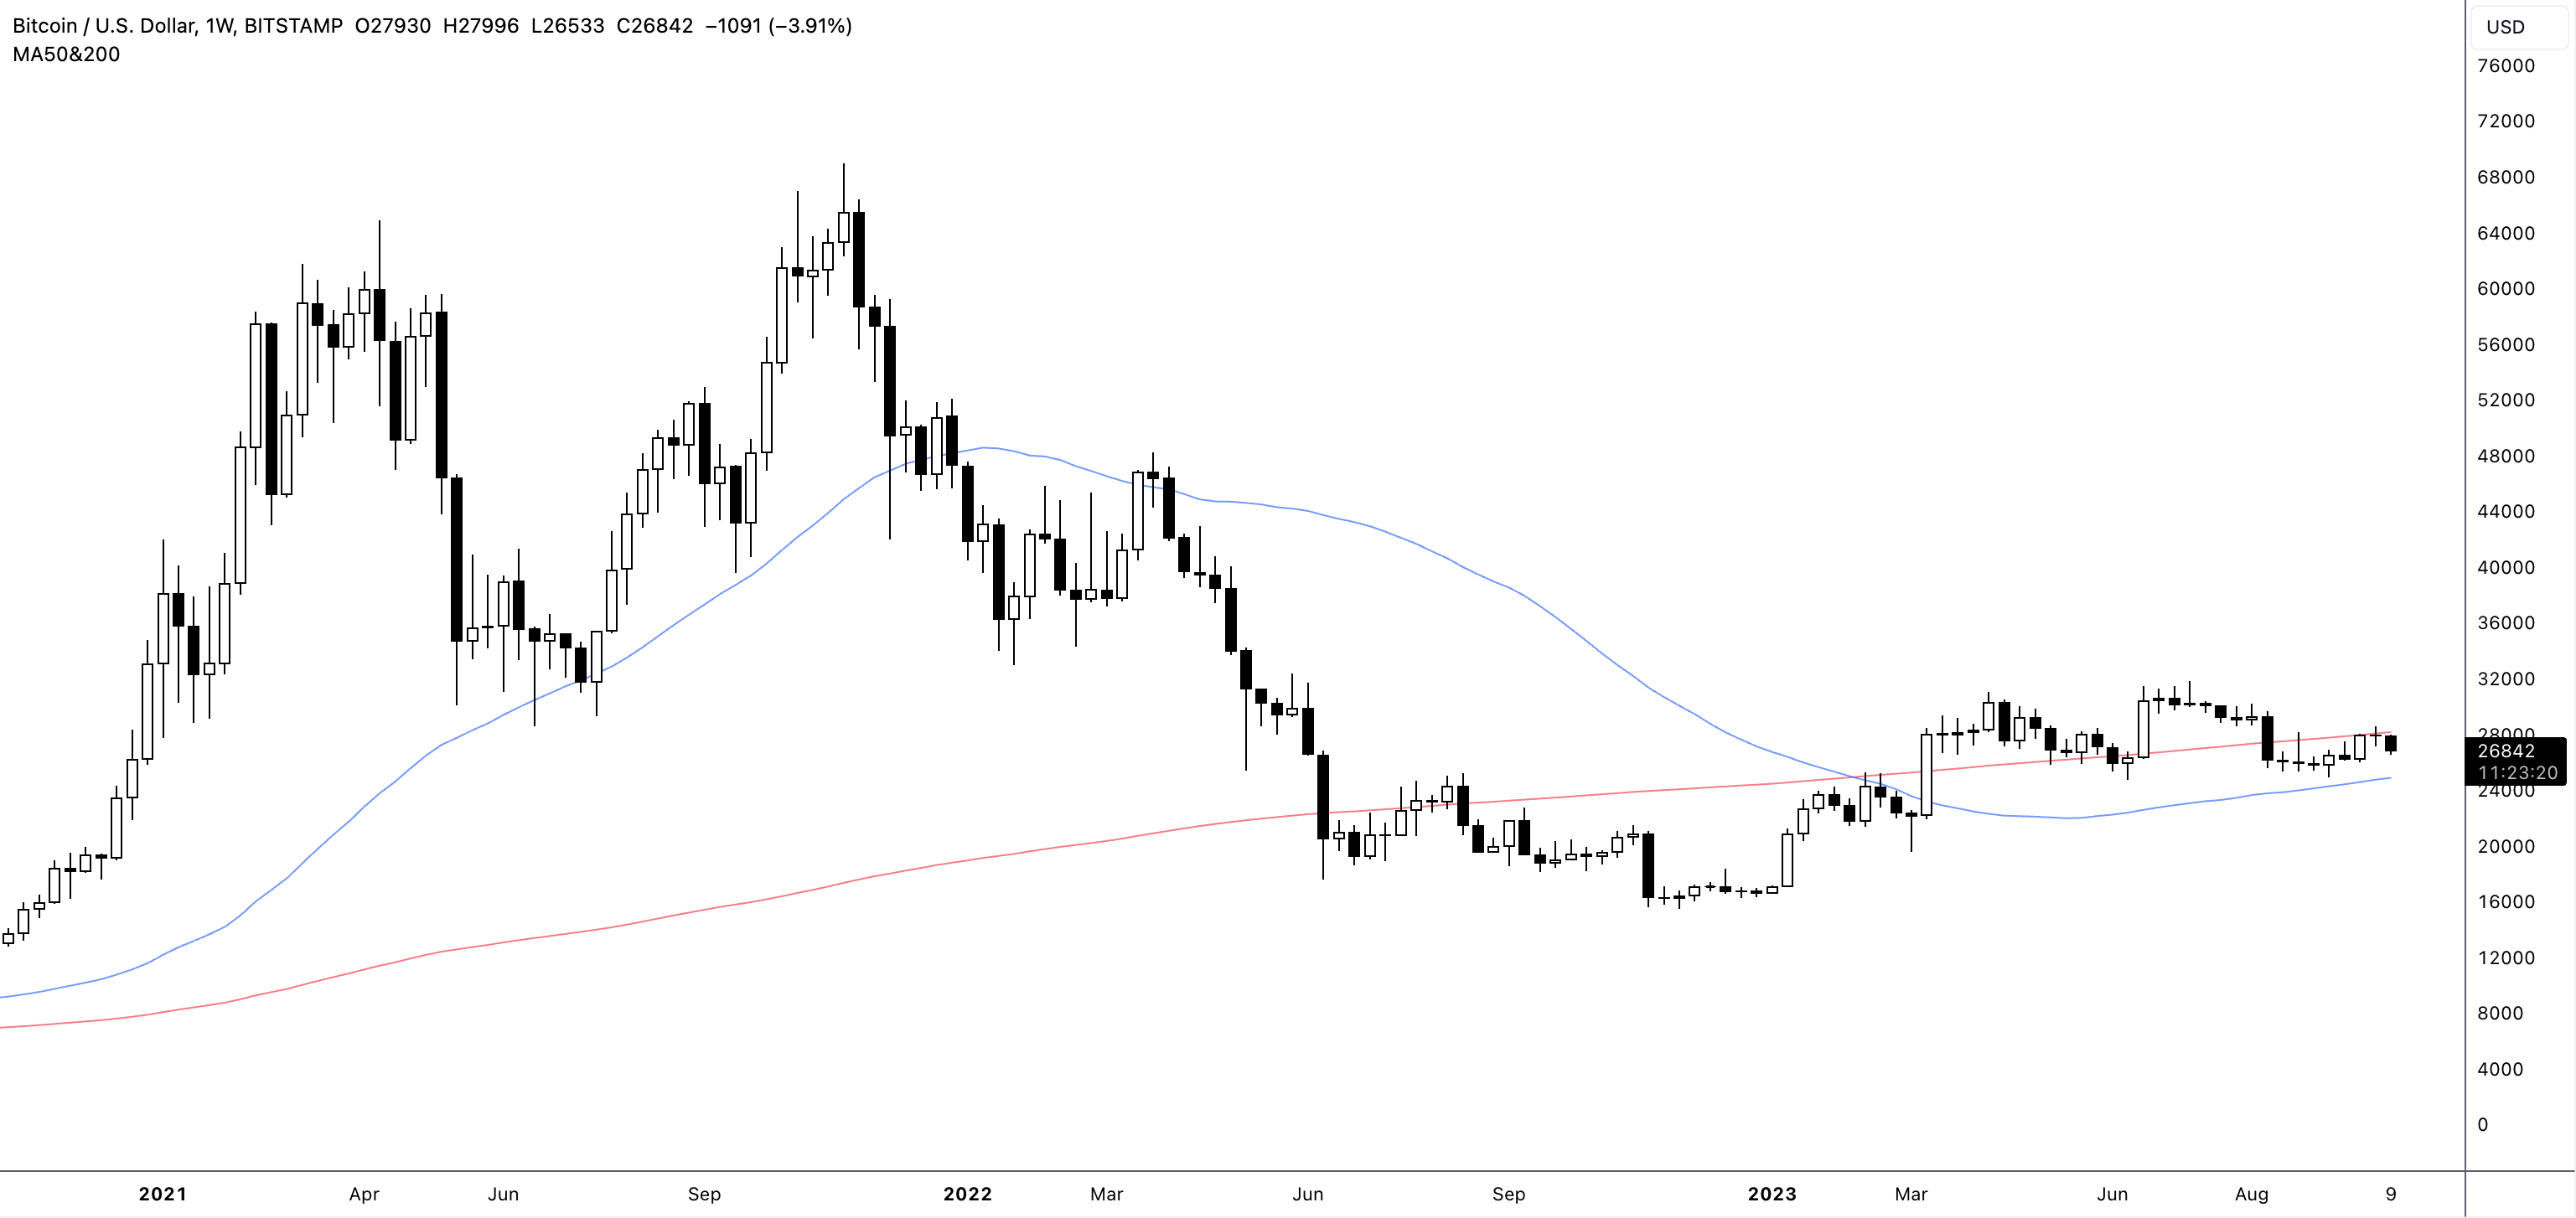
\includegraphics[width=\textwidth]{./assets/img/bitcoin_moving_averages.png}
    \caption{Figure shows the 50-day \gls{ema} in blue and the 200-day \gls{ema} in red applied to \gls{btc} on a weekly \gls{tf} from October 2020 to October 2023.}
    \label{fig:bitcoin_moving_averages}
\end{figure}

% Bollinger Bands
\subsection{Bollinger Bands}
\label{sub:BB}
John Bollinger developed the \gls{bb} in the early 1980's, building on the work of several earlier researchers. These include Wilfrid Ledoux's work on trading bands in 1960, Chester Keltner's introduction of the Keltner channel \citep{keltner1960make}, J.M. Hurst's studies involving graphical representations of price structures, the popularisation of percentage bands in the 1970's (whose specific origin remains unknown), and Richard Donchian's contribution with the Donchian channels \citep{bollinger2023}.
\newline
\newline
\gls{bb} are used to asses the relative highs and lows of an asset's price. They are made up of two bands, each representing a positive and negative \gls{std} from a 20-day \gls{sma}. These bands allow traders to identify potential overbought conditions, indicated by prices continuously touching the upper band, known as $\text{BOLU}$, and oversold conditions, indicated by prices continuously touching the lower band, known as $\text{BOLD}$. See figure \ref{fig:bollinger_bands} for an illustration.

\begin{figure}[ht]
    \centering
    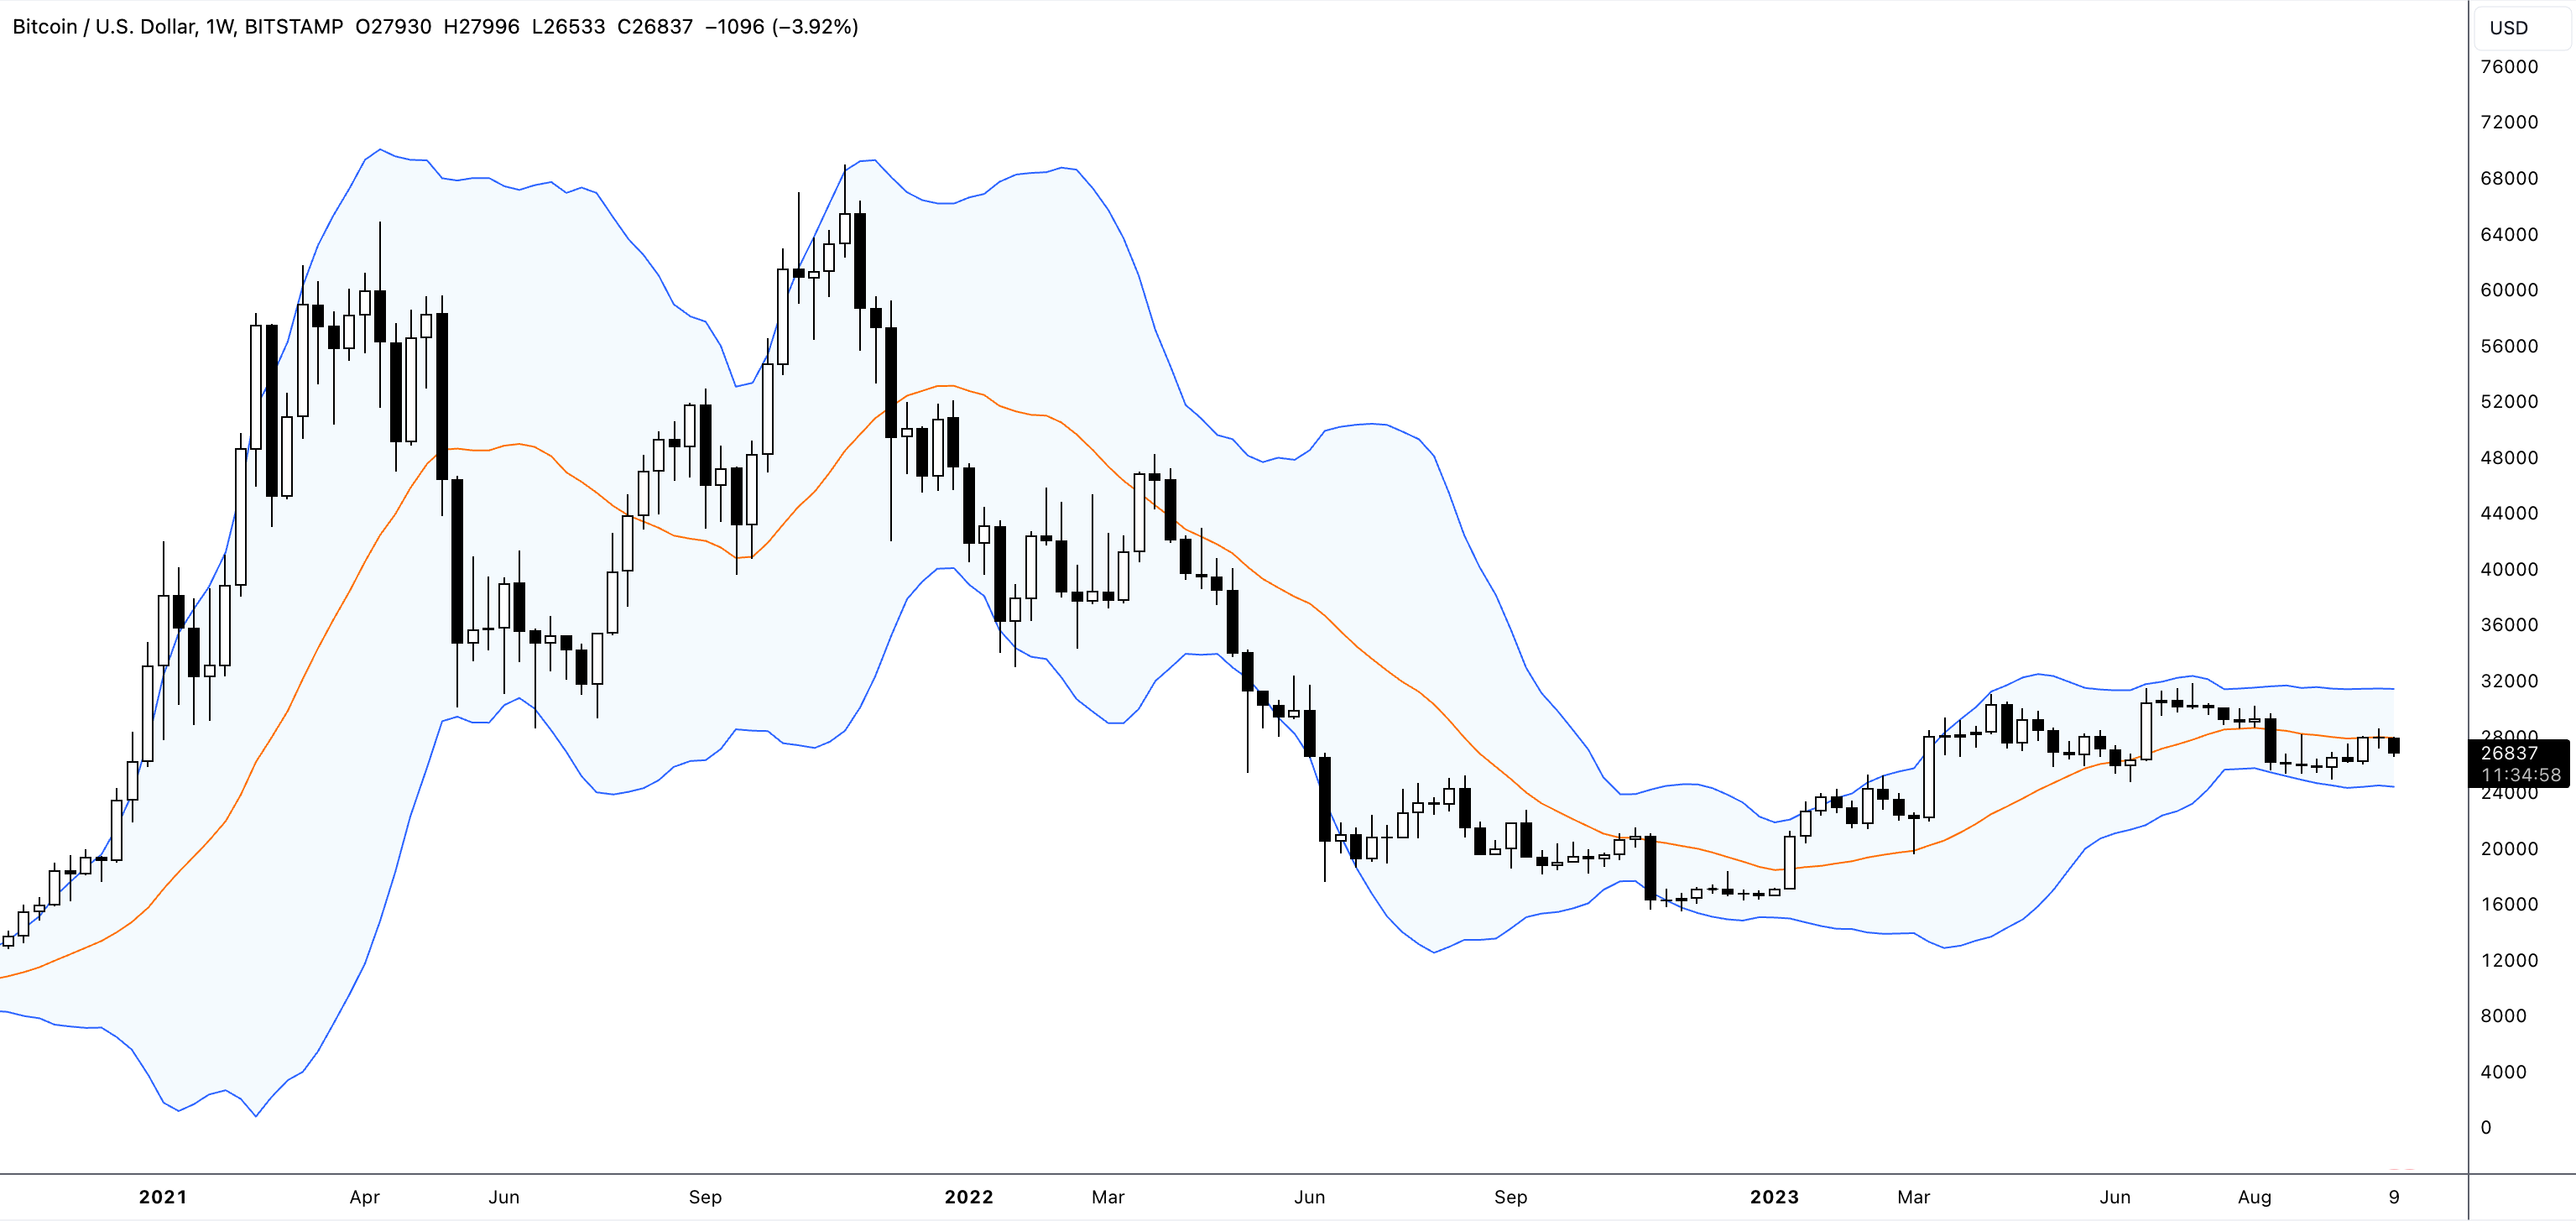
\includegraphics[width=\textwidth]{./assets/img/bitcoin_bollinger_bands.png}
    \caption{Figure shows the \gls{bb} applied to \gls{btc} on a weekly \gls{tf} from October 2020 to October 2023.}
    \label{fig:bollinger_bands}
\end{figure}

\noindent
The upper bands are calculated using the equation \ref{eq:bb_upper_band} and the lower bands using the equation \ref{eq:bb_lower_band}. Where, the \gls{tp} can be calculated by (High + Low + Close) / 3), $n$ is the number of days in the smoothing period, $m$ the number of \glspl{std} and $\sigma [\text{TP}, n]$ the \gls{std} over the last $n$ periods of \gls{tp}.

\myequations{Computing the upper Bollinger Band}
\begin{equation}
    \centering
    \text{BOLU} = \text{MA}(\text{TP}, n) + m \cdot \sigma [\text{TP}, n]
    \label{eq:bb_upper_band}
\end{equation}

\myequations{Computing the lower Bollinger Band}
\begin{equation}
    \centering
    \text{BOLD} = \text{MA}(\text{TP}, n) - m \cdot \sigma [\text{TP}, n] 
    \label{eq:bb_lower_band}
\end{equation}

% Relative Strength Index
\subsection{Relative Strength Index}
\label{sub:RSI}
The \gls{rsi} is a momentum indicator developed by J. Welles Wilder Jr. and first introduced in 1978 in his book \textit{New Concepts in Technical Trading Systems} \citep{Wilder_1978}. Its primary purpose is to measure the speed and magnitude of recent price changes in an asset, providing an indication of whether an asset is currently overbought or oversold on a scale of zero to 100. In the context of the \gls{rsi}, the standard overbought and oversold thresholds are typically set at 70 and 30 respectively, with values above 70 indicating overbought conditions and values below 30 indicating oversold conditions.
\newline
\newline
The \gls{rsi} is calculated using equation \ref{eq:relative_strength_index}. The \gls{rs} is obtained through a three-step calculation process. Firstly, the average daily percentage gains and losses over a predetermined look-back period $n$ of typically 14 days, are computed. Subsequently, the averages of previously calculated gains and losses are multiplied by $n-1$, and the current daily percentage gain or loss is added to emphasize the present price trends. The gain and loss calculations are divided by $n$ to receive their respective arithmetic mean. This computation is commonly referred to as \gls{smma}. Finally, the ratio between the computed \gls{smma} of the gain and loss yields the value of $\text{RS}$.

\myequations{Computing the Relative Strength Index}
\begin{equation}
    \centering
    \text{RSI} = 100 - \frac{100}{1 + \text{RS}}
    \label{eq:relative_strength_index}
\end{equation}

\begin{figure}[ht]
    \centering
    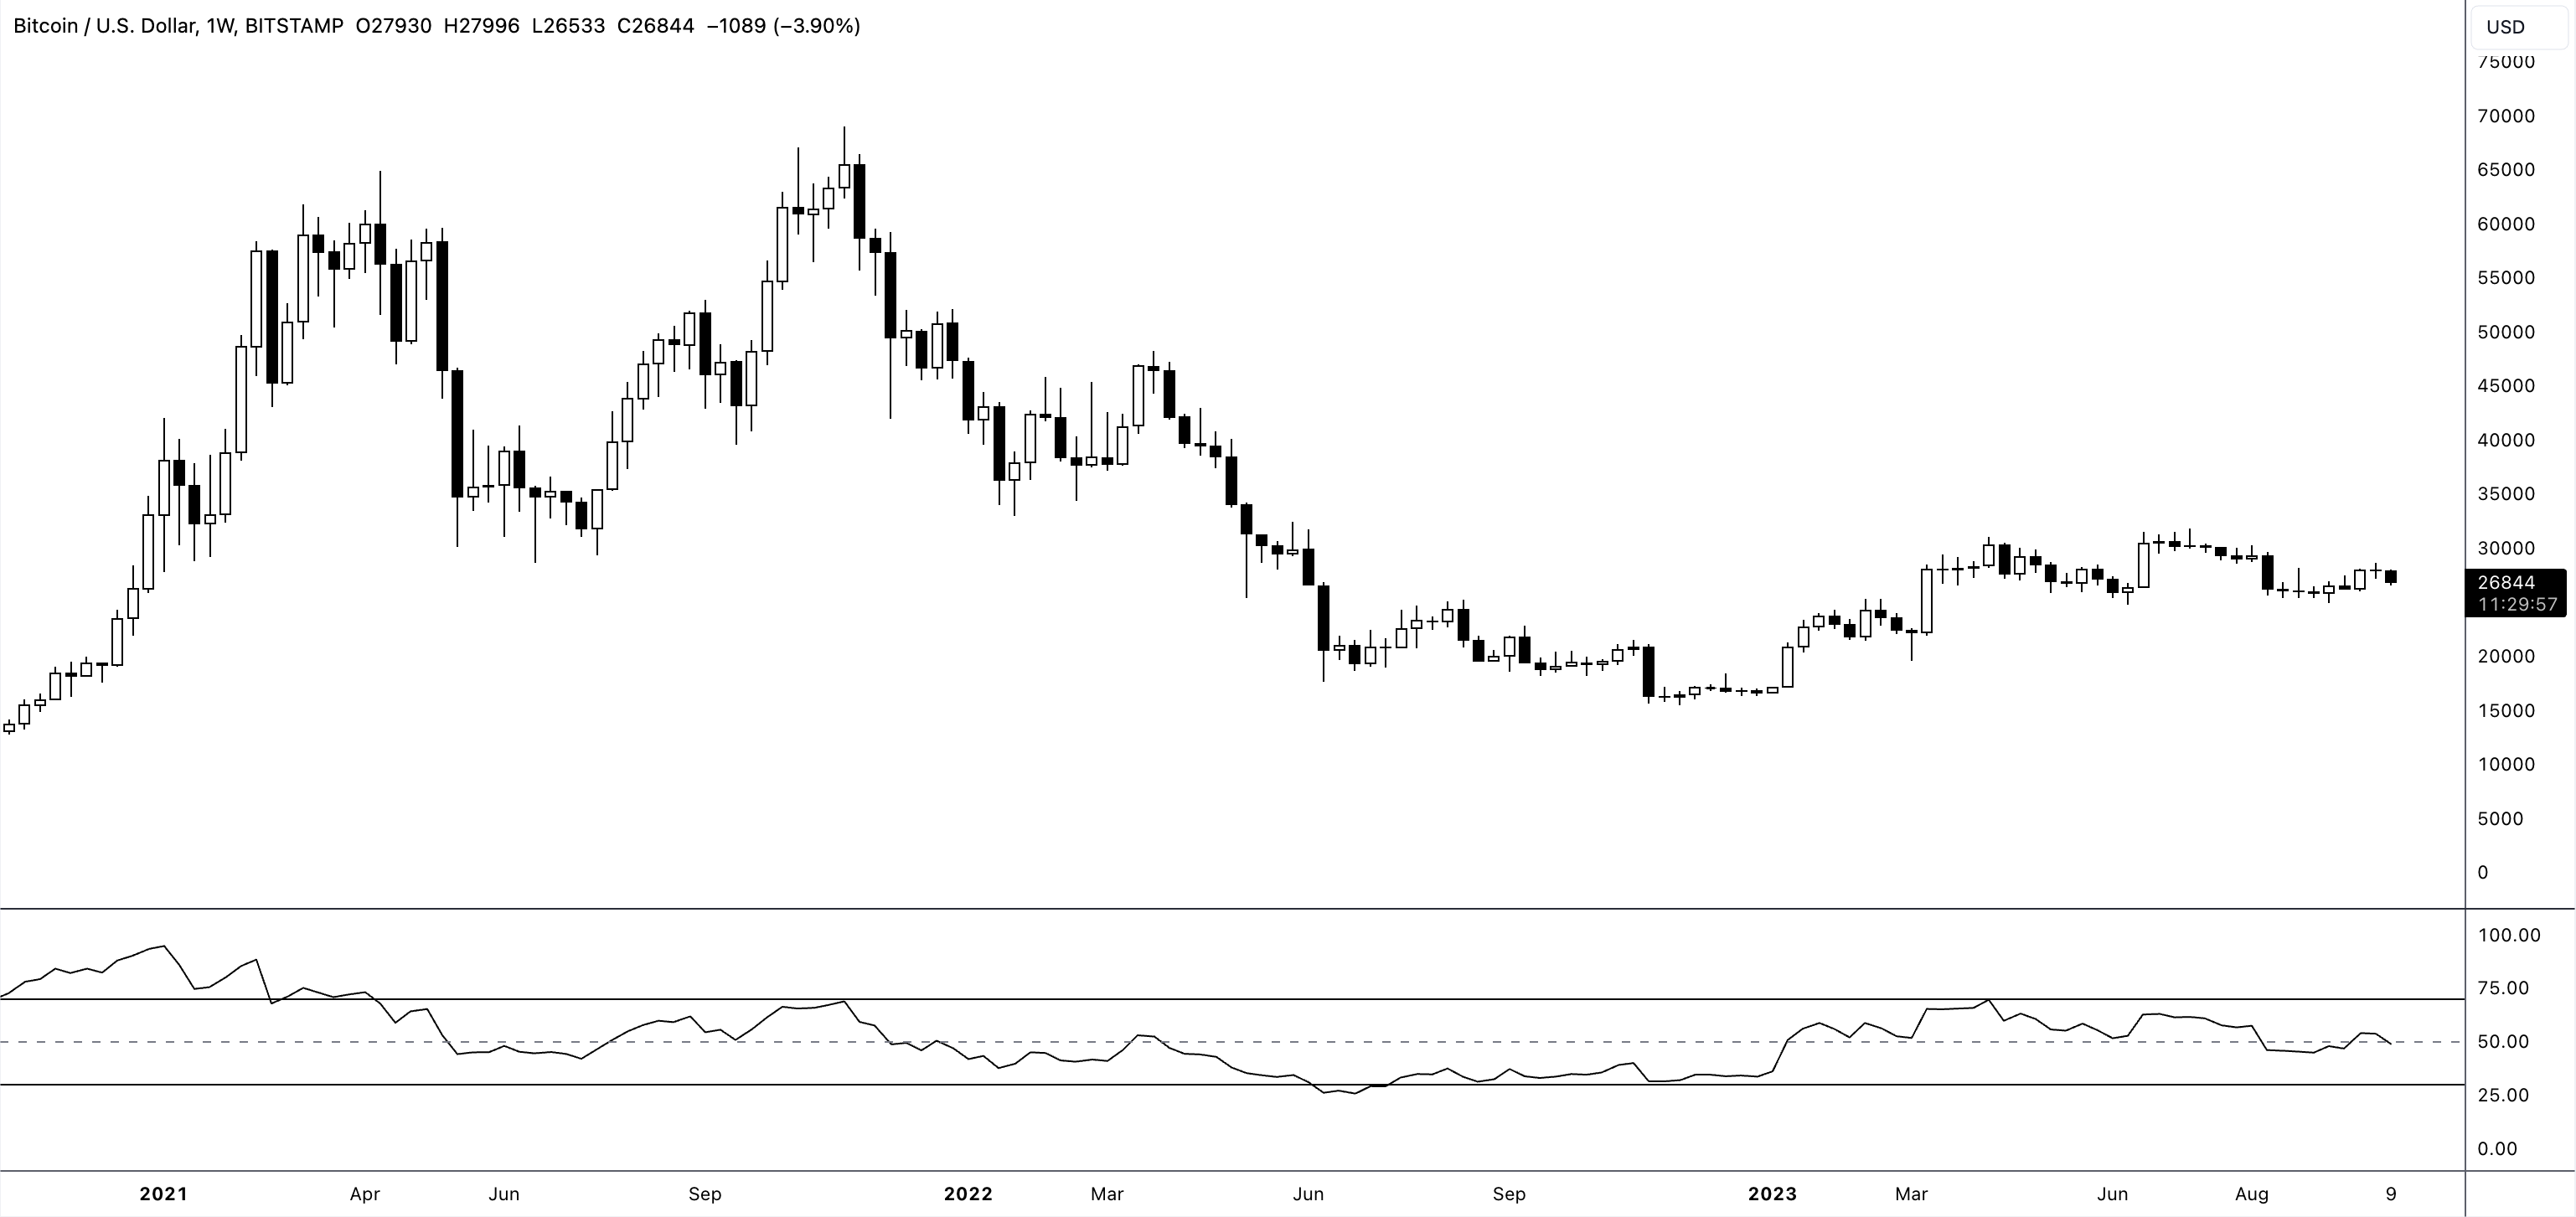
\includegraphics[width=\textwidth]{./assets/img/bitcoin_rsi.png}
    \caption{Figure shows the \gls{rsi} applied to \gls{btc} on a weekly \gls{tf} from October 2020 to October 2023.}
    \label{fig:relative_strength_index}
\end{figure}

% MACD
\subsection{Moving Average Convergence Divergence}
\label{sub:MACD}
Determining the precise origins of the \gls{macd} indicator is difficult, as even its inventor, Gerald Appel, remains vague in his 2005 book \textit{Technical Analysis: Power Tools for Active Investors}. Appel states that the \gls{macd} was developed in the late 1970s, although he does not cite any specific sources \citep{appel2005technical}. However, it is evident that his 1985 report, titled \textit{The Moving Average Convergence-divergence Trading Method: Advanced Version} \citep{appel1985moving} is a refined version of his initial work on the \gls{macd}.
\newline
\newline
The \gls{macd} is a tool used by traders to objectively monitor the correlation between two distinct \glspl{ma}. Fundamentally, the \gls{macd} is comprised of the difference between a faster \gls{ma} (representative of short-term market trends) and a slower \gls{ma} (reflecting longer-term trends). According to the tech report \textit{A Quick Tutorial in MACD: Basic Concepts}, Appel uses two separate sets of \glspl{ma} to calculate \glspl{macd} \citep{appel2008quick}. One set includes a 26-day and 12-day \gls{ema}, while the other set consists of a 39-day and 19-day \gls{ema}. Equation \ref{eq:macd} employs the 26-day and 12-day \gls{ema} in the calculation of the \gls{macd}. Furthermore, the \gls{macd} incorporates a signal line, which typically uses the 9-day \gls{ema} of the \gls{macd} line.

\myequations{Computing the Moving Average Convergence Divergence}
\begin{equation}
    \centering
    \text{MACD} = \text{12-Period} \text{ EMA} - \text{26-Period} \text{ EMA}
    \label{eq:macd}
\end{equation}

\noindent
When the short-term average is higher than the long-term average, the \gls{macd} signals upward momentum. On the other hand, when the short-term average drops below the long-term average, it signals downward momentum as illustrated in figure \ref{fig:macd_momentum}

\begin{figure}[ht]
    \centering
    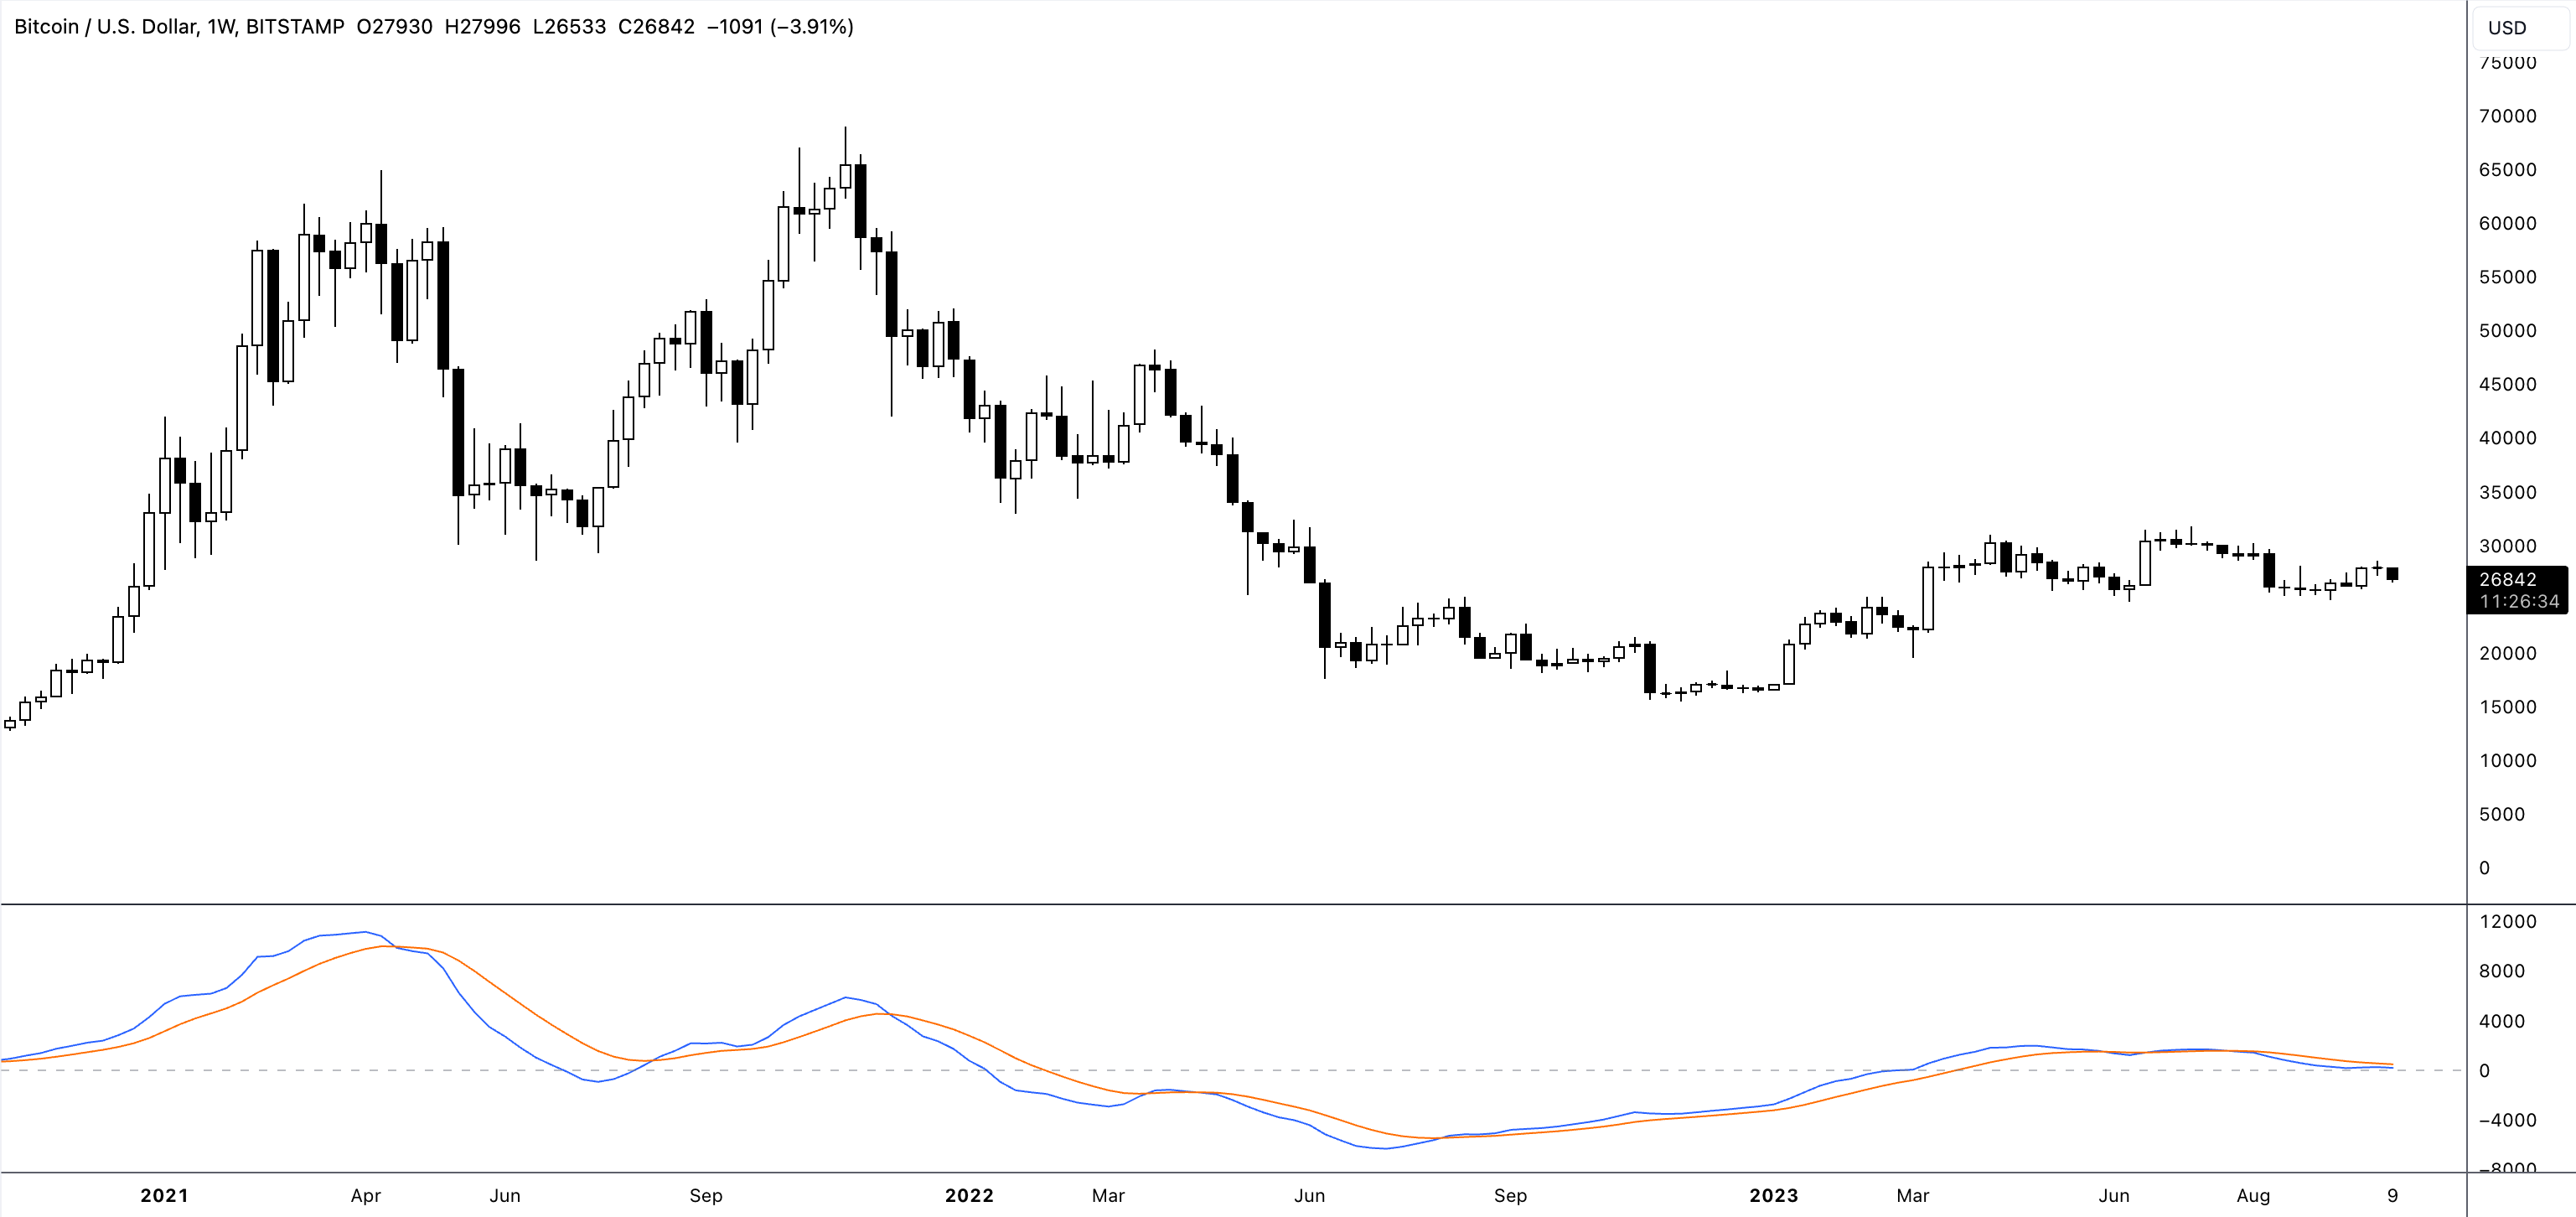
\includegraphics[width=\textwidth]{./assets/img/bitcoin_macd.png}
    \caption{Figure shows the \gls{macd} applied to \gls{btc} on a weekly \gls{tf} from October 2020 to October 2023.}
    \label{fig:macd_momentum}
\end{figure}

% CCI
\subsection{Commodity Channel Index}
\label{sub:CCI}
Originally developed by Donald Lambert and introduced in his book \textit{Commodity Channel Index: Tools for Trading Cyclical Trends} \citep{lambert1983commodity}, the \gls{cci} is an oscillator that has gained considerable popularity since its inception. While initially designed for commodities, it has evolved into a widely used technical indicator for assessing cyclical trends in equities and currencies.
\newline
\newline
Like many oscillators, the primary purpose of the \gls{cci} is to identify overbought (above +100) and oversold (below -100) levels in the market. This is achieved by measuring the deviation of an asset's \gls{tp} (see section \ref{sub:BB}) from its statistical average over a specific period, often using the 20-day \gls{sma}. Equation \ref{eq:cci} outlines the calculation of the \gls{cci}, where $n$ is the number of periods. The formula in the denominator calculates the mean deviation, i.e., the absolute difference between each typical price and the \gls{sma} over $n$ periods.

\myequations{Calculation of the Commodity Channel Index}
\begin{equation}
    \centering
    \text{CCI} = \frac{\text{TP} - \text{ SMA}}{0.015 \cdot \frac{\sum_{i=1}^n | \text{TP}_i - \text{ SMA} |}{n}}
    \label{eq:cci}
\end{equation}

\begin{figure}[ht]
    \centering
    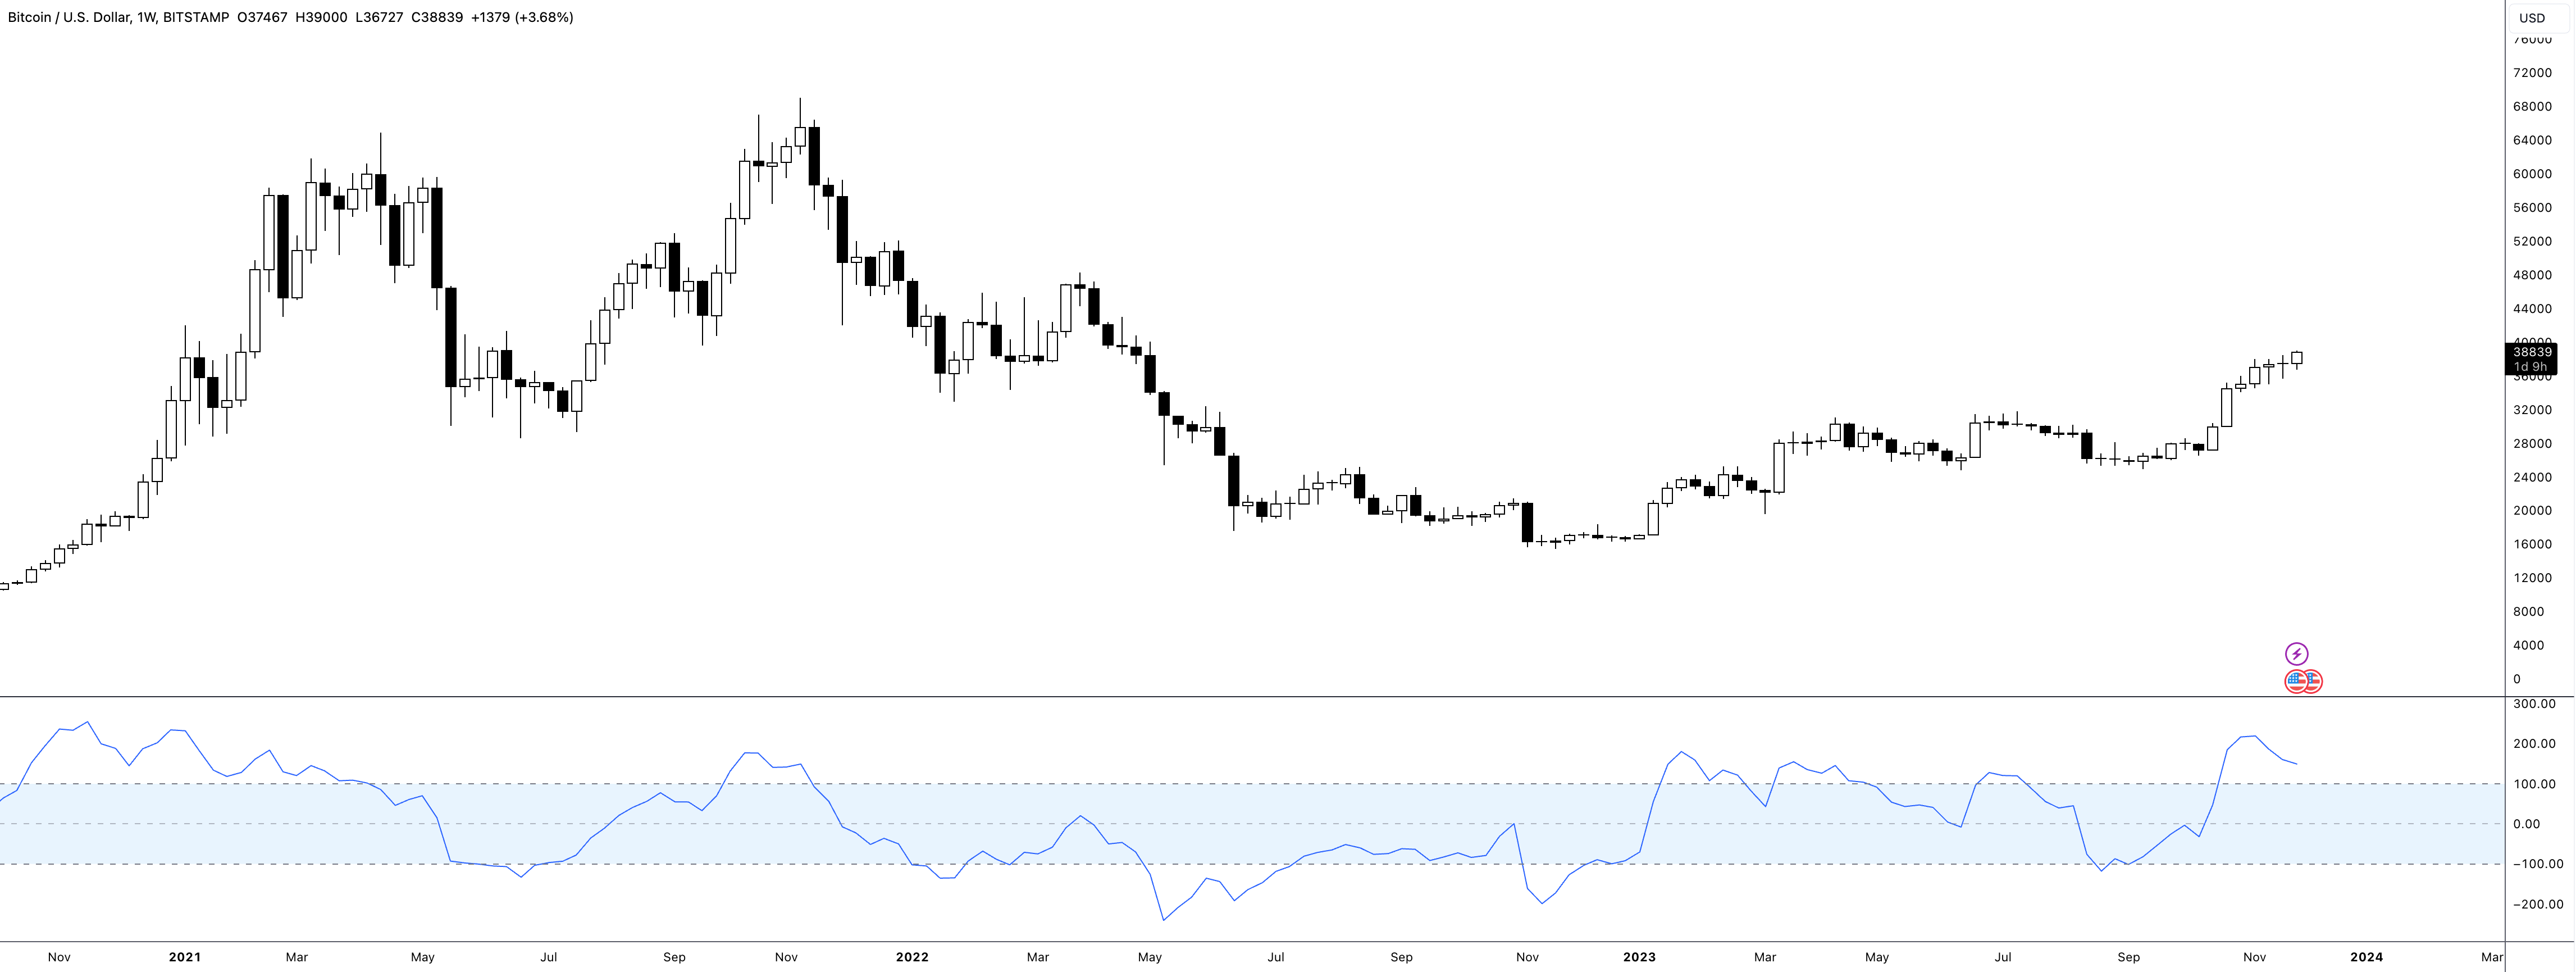
\includegraphics[width=\textwidth]{./assets/img/btc-cci.png}
    \caption{Figure shows the \gls{cci} applied to \gls{btc} on a weekly \gls{tf} from October 2020 to December 2023.}
    \label{fig:cci}
\end{figure}

% OBV
\subsection{On-Balance Volume}
\label{sub:OBV}
Joseph Granville introduced \gls{obv} in 1963 in his book \textit{Granville's New Key to Stock Market Profits} \citep{granville1963new}. As a momentum indicator, \gls{obv} uses volume flow to anticipate changes in the price of an asset.
\newline
\newline
Granville's concept was based on the belief that volume plays a central role in market dynamics. The \gls{obv} was designed to predict major market movements by examining shifts in volume. Grandville argued that a significant increase in volume, unaccompanied by a significant change in price, would eventually lead to an upward or downward price movement.
\newline
\newline
The calculation of $\text{OBV}_t$ is determined by equation \ref{eq:obv}. It involves adding $\text{OBV}_{t-1}$ and either the current volume, zero, or the negative of the current volume, depending on the relationship between the closing price at time $t$ and $t-1$.

\myequations{Calculation of the On-Balance Volume}
\begin{equation}
    \centering
    \text{OBV}_t = \text{OBV}_{t-1} + \left\{ \begin{array}{rcl}
    \text{volume,} \quad \text{if close}_t > \text{close}_{t-1} \\
    0, \quad \text{if close}_t = \text{close}_{t-1} \\
    \text{-volume,} \quad \text{if close}_t < \text{close}_{t-1}
    \end{array}\right.
    \label{eq:obv}
\end{equation}

\noindent
The theory behind \gls{obv} revolves around the distinction between smart money (institutional investors) and less sophisticated retail investors. When institutional investors buy an asset that retail investors are selling, volume can increase even if the price remains relatively stable. Eventually, the increased volume drives the price up. As larger investors begin to sell, smaller investors begin to buy.
\newline
\newline
Analysts use \gls{obv} volume figures to track large institutional investors, often referred to as smart money, treating divergences between volume and price as indicators of the relationship between smart money and the broader market. Such divergences can signal opportunities to trade against prevailing trends, highlighting instances where smart money is driving up prices before strategically selling.

\begin{figure}[ht]
    \centering
    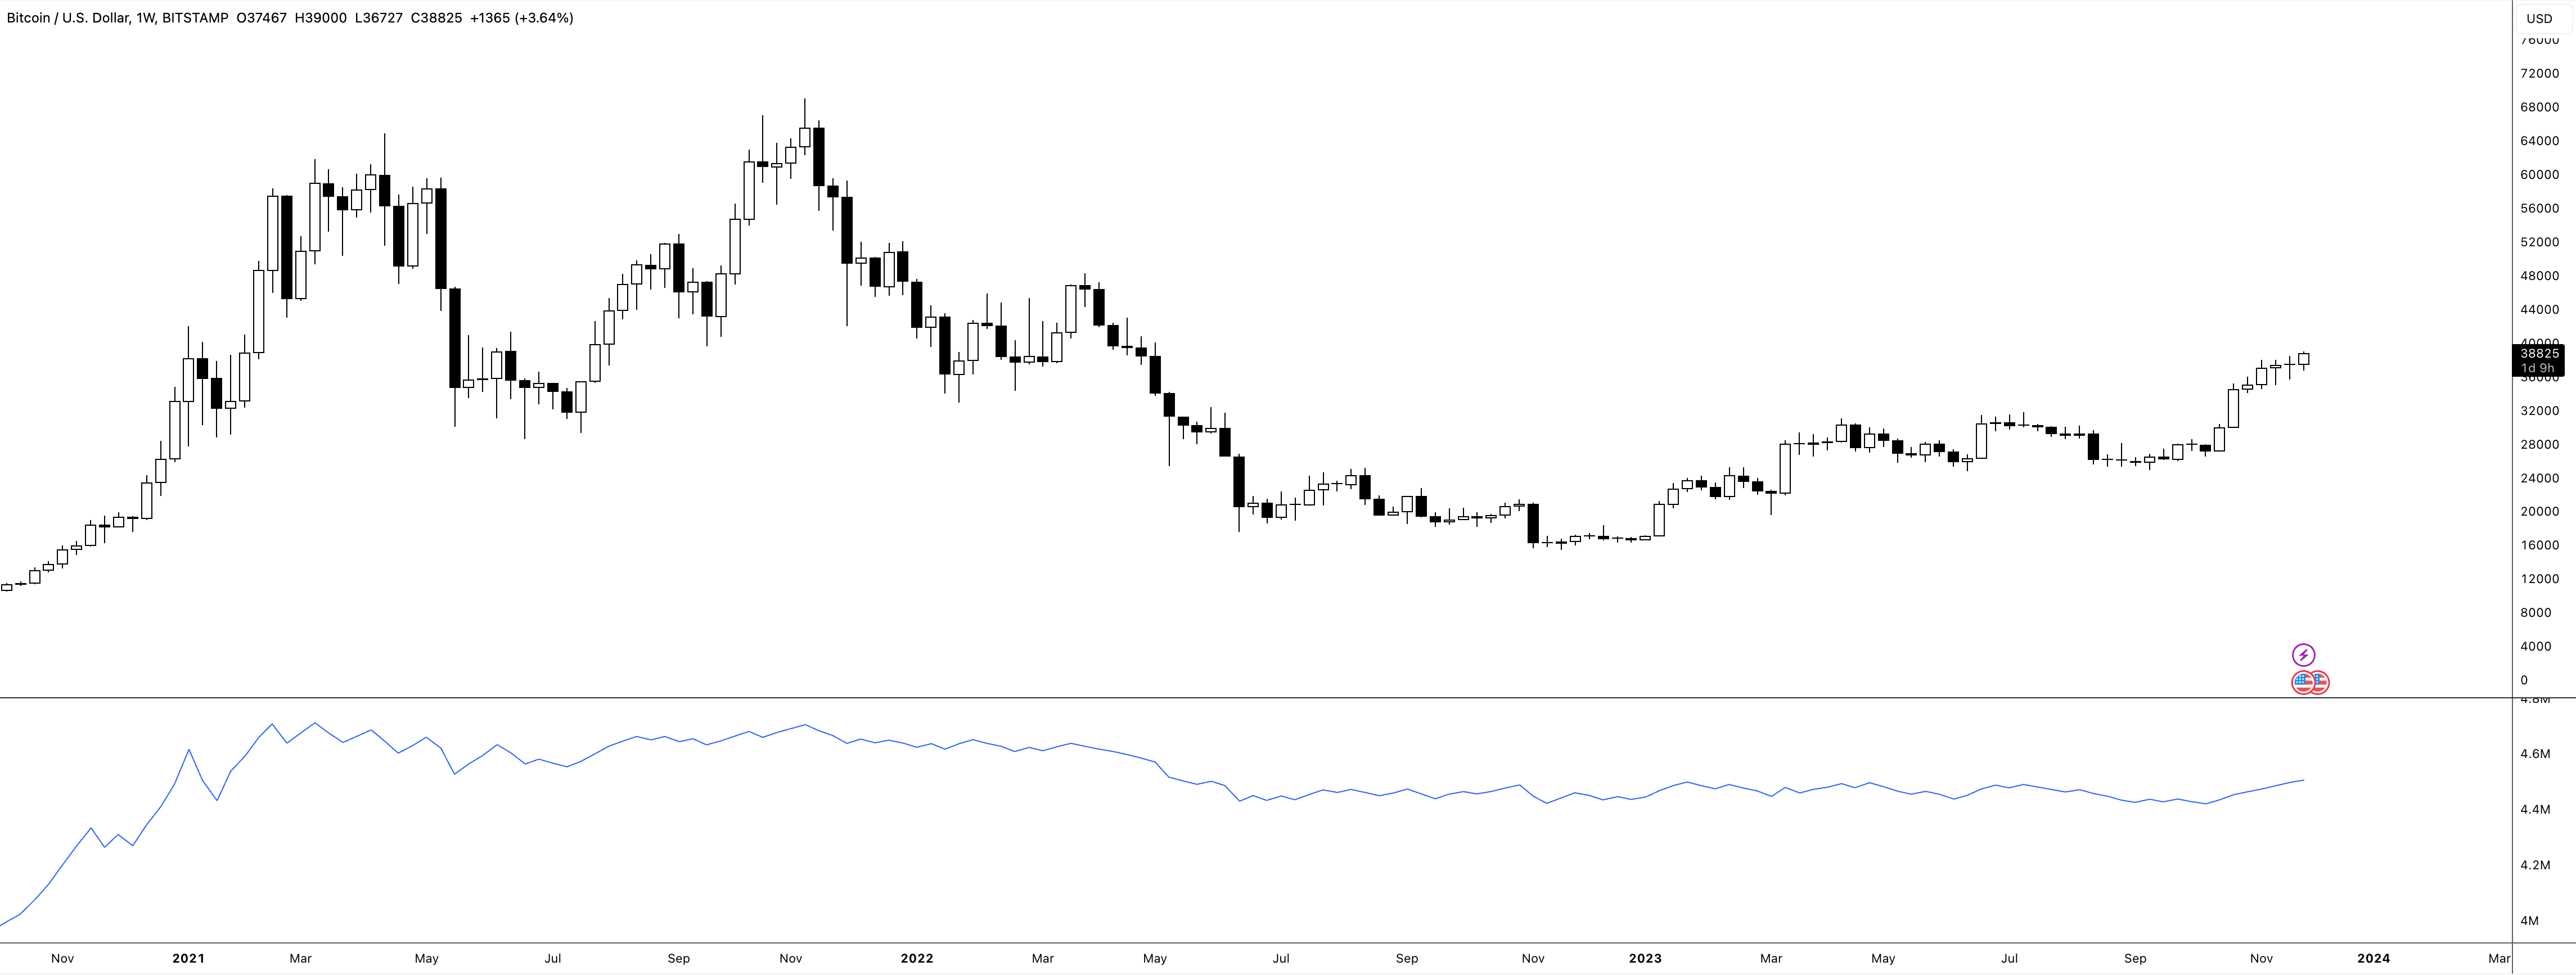
\includegraphics[width=\textwidth]{./assets/img/btc-obv.png}
    \caption{Figure shows the \gls{obv} applied to \gls{btc} on a weekly \gls{tf} from October 2020 to December 2023.}
    \label{fig:obv}
\end{figure}

% AD
\subsection{Accumulation/Distribution Indicator}
\label{sub:AD}

% Introduction
Market analyst Marc Chaikin developed the \gls{ad} to measure the cumulative flow of money into or out of an asset. This indicator provides valuable insight into the complex relationship between price and volume dynamics \citep{Yu_2023}.
\newline
\newline
% Equation
The calculation of the \gls{ad} involves three steps. First, the \gls{mfm} is calculated using the equation \ref{eq:MFM}, where $\text{close}$ is the closing price and $\text{low}$ and $\text{high}$ are the corresponding lowest and highest prices achieved during the period. Secondly, the \gls{mfv} is calculated by multiplying the \gls{mfm} by the current volume. Finally, the current \gls{ad} is calculated by multiplying the previous \gls{ad} by the \gls{mfv}.

\myequations{Calculation of the Money Flow Multiplier}
\begin{equation}
    \centering
    \text{MFM} = \frac{\text{(Close - Low) - (High - Close)}}{\text{High - Low}}
    \label{eq:MFM}
\end{equation}

\noindent
% Interpretation
A rising \gls{ad} line indicates accumulation (buying pressure), while falling \gls{ad} indicates distribution (selling pressure). Traders use these trends to anticipate potential price movements and assess the strength of ongoing trends based on volume and the direction of the trend.

\begin{description}
    \item[Uptrends:] A rising \gls{ad} line confirms strong support for the uptrend and indicates sufficient money flow.
    \item[Downtrends:] A falling \gls{ad} line in downtrends indicates support for the downtrend, reflecting money flowing out of the asset.
    \item[Uptrend divergence:] When the \gls{ad} line falls during an uptrend, it indicates a divergence. This may indicate that the rise in the assets price lacks strong support from accumulation volume and may signal a reversal.
    \item[Downtrend divergence:] In a downtrend with a rising \gls{ad} line, distribution volume may be decreasing, possibly signalling a reversal.
\end{description}

\begin{figure}[ht]
    \centering
    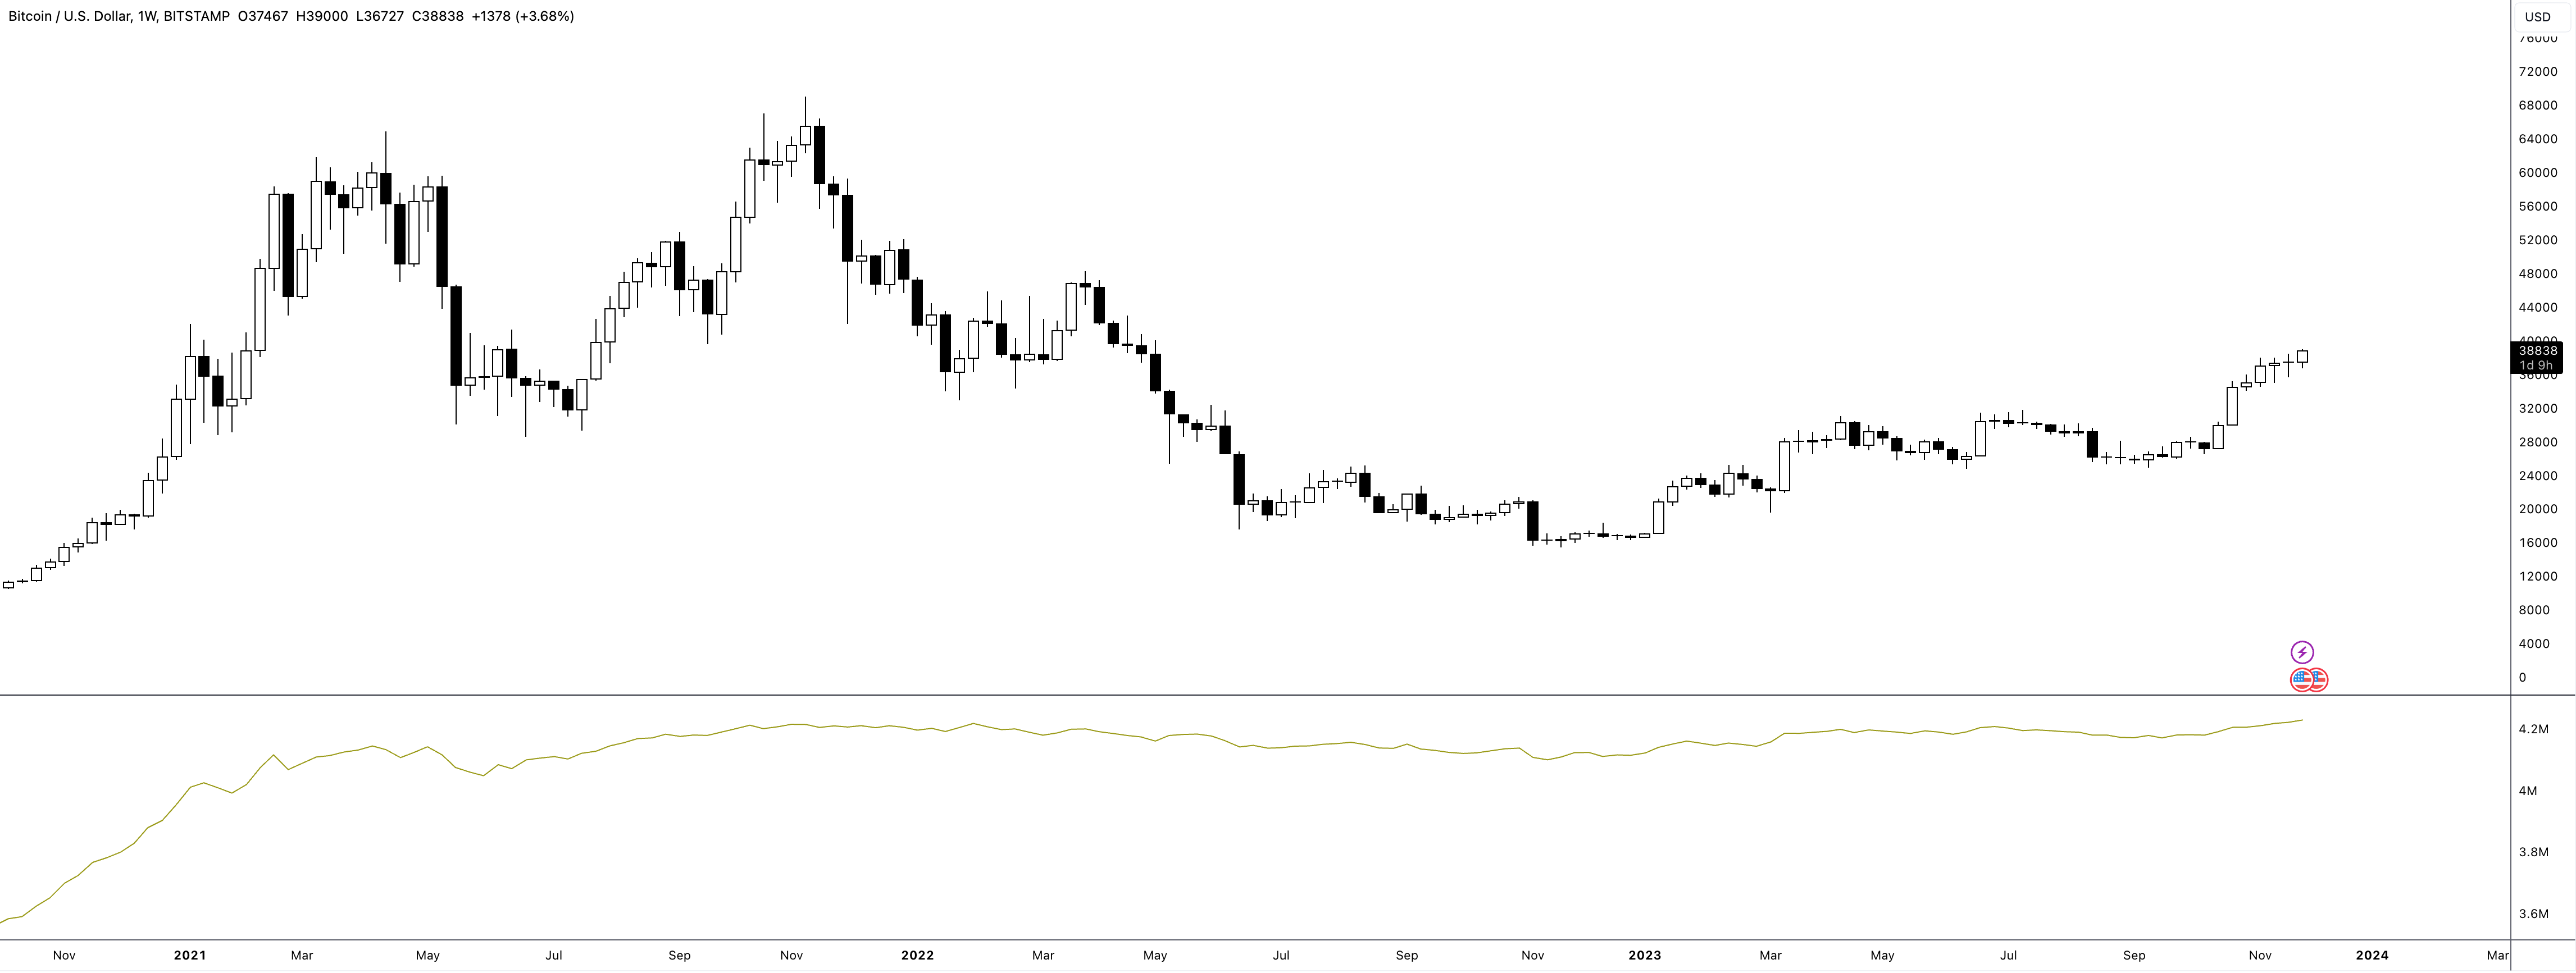
\includegraphics[width=\textwidth]{./assets/img/btc-ad.png}
    \caption{Figure shows the \gls{ad} applied to \gls{btc} on a weekly \gls{tf} from October 2020 to December 2023.}
    \label{fig:ad}
\end{figure}

% ADX
\subsection{Average Directional Index}
\label{sub:ADX}
In addition to the \gls{rsi}, J. Welles Wilder Jr. introduced the \gls{adx} in his book \textit{New Concepts in Technical Trading Systems} \citep{Wilder_1978} in 1978. Unlike the \gls{rsi}, the \gls{adx} is a lagging indicator and is derived from two other indicators developed by J. Welles Wilder Jr. namely the \gls{+di} and the \gls{-di}. The \gls{adx} combines these indicators and smooths the result with a \gls{ma}.
\newline
\newline
To calculate the \gls{+di}, a smoothing period is defined (usually set at 14 days, as suggested by J. Welles Wilder Jr. in his book). The \gls{+di} is obtained by subtracting the previous high from the current high for the period, dividing the result by the true range for the period, and multiplying it by 100. The true range is defined as the largest of the following: the current high minus the current low, the current high minus the previous close, or the absolute value of the current low minus the previous close.
\newline
\newline
Similarly, the \gls{-di} is calculated by selecting a smoothing period, subtracting the current low from the previous low for the period, dividing it by the true range for the given period, and multiplying the result by 100. The \gls{dmi} is then calculated by subtracting \gls{-di} from \gls{+di}, dividing the absolute value of this result by the absolute sum of \gls{+di} and \gls{-di}, and multiplying by 100.
\newline
\newline
To obtain the first \gls{adx}, the \gls{dmi} is calculated for 14 periods. The equation \ref{eq:Average_Directional_Index} then calculates the subsequent \glspl{adx}.

\myequations{Average Directional Index}
\begin{equation}
    \centering
    \text{\gls{adx}} = \frac{(\text{Prior ADX} \cdot 13) + \text{Current ADX}}{14}
    \label{eq:Average_Directional_Index}
\end{equation}

\begin{figure}[ht]
    \centering
    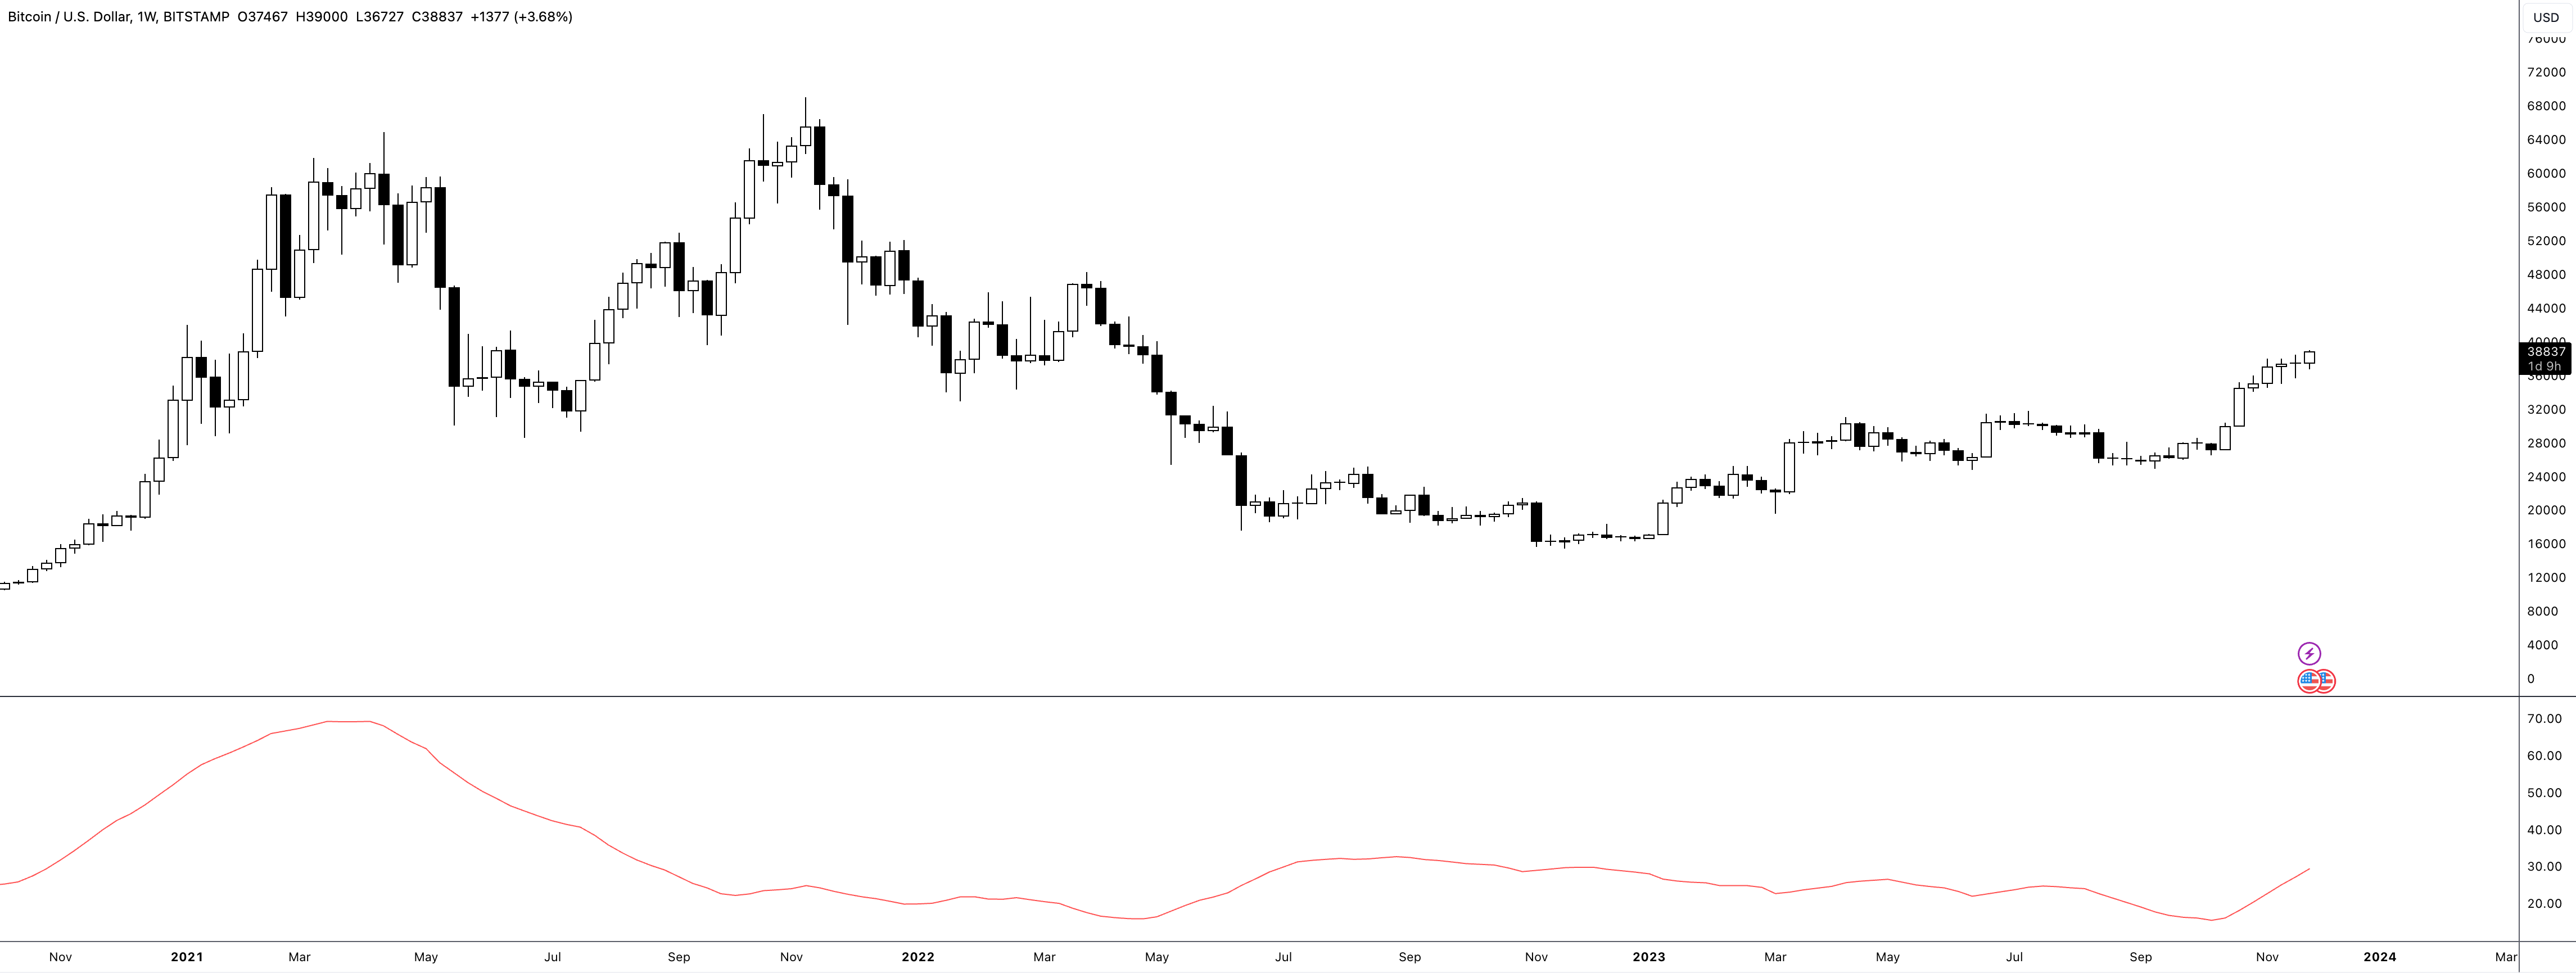
\includegraphics[width=\textwidth]{./assets/img/btc-adx.png}
    \caption{Figure shows the \gls{adx} applied to \gls{btc} on a weekly \gls{tf} from October 2020 to December 2023.}
    \label{fig:adx}
\end{figure}

\noindent
The \gls{adx} is a valuable tool for investors to assess the strength of a trend, while the \gls{+di} and \gls{-di} help to determine the direction of a trend.
\newline
\newline
The \gls{adx} is useful in determining the strength of a trend. A reading above 25 indicates a strong trend, while a reading below 20 indicates a weaker trend. Trading signals can be generated by crossing the \gls{-di} and \gls{+di} lines. For example, if the \gls{+di} crosses the \gls{-di} and the \gls{adx} is above 20, this signals a potential buying opportunity. Conversely, if the \gls{-di} crosses the \gls{+di} and the \gls{adx} is above 20, this is an opportunity to go short.
\newline
\newline
These crosses also guide exit strategies for existing trades. For example, in a long position, consider exiting when the \gls{-di} crosses above the \gls{+di}. In addition, a \gls{adx} reading below 20 indicates a trendless market, suggesting caution in entering new trades during such periods.

% TA-Lib
\subsection{TA-Lib}
\label{sub:TA-Lib}
TA-Lib is a widely used Python package for technical analysis of financial market data. It offers over 200 technical indicators and also candlestick-pattern recognition, which will not be used in this thesis. Installing TA-Lib on any device is straightforward and requires the us of HomeBrew and PIP for installation.\footnote{https://ta-lib.github.io/ta-lib-python/install.html, accessed on 06.10.2023}

\begin{verbatim}
    brew install ta-lib
\end{verbatim}

\begin{verbatim}
    pip install TA-Lib
\end{verbatim}